% !TEX root = ../thesis.tex

\chapter{Syntactic part} \label{sec:methodology}
Based on the Analytical part~\ref{sec:analytical} let us create a mathematical models to predict customer behavior consist of
vendor, psychology and loyalty sub-models (Described in own section ~\ref{sec:submodels}) combined in Hidden markov model (HMM) to final prediction model.
Hidden states in the HMM produced in readable format by viterbi algoritm (See section Viterbi~\ref{subsec:viterbi}) we used for orders calculation for final income prediction.
Viterbi serve us the state with the most probability during propagation true HMM.
We lead up to get a better results than actual standard statistical regression methods~\ref{sec:regression} to predict customer behavior in e-commerce.
In the final our model will return future income for online store based on previous data with better aberration than linear or polynomial regression has.
For successfully prediction open data for store strength and customer satisfaction and some predefined and computed variables from store will be used.
\section{Modeling prediction of customer behavior} \label{sec:modeling}
Let us the model to store information about successfully order prediction.
In the same way the model is able to predict where the customer leaves the store, but this situation was not added to our prediction experiment~\ref{experiment}
Then based on that prediction data, calculation of future income for store were done.
Our designed model is consists of three sub-models, which are partially dependent on each other.
Vendor ,\ psychology and loyalty models we created for our prediction to simulate customer behavior.
Then partial results was combined to complex prediction mechanism, as you can see on figure~\ref{Model schema with interaction}.
As a combination method Hidden Markov model was selected as appropriate.
HMM in combination with Viterbi algorithm will be used to detect hidden states, which will be reflected predefined weights for specific industries,
to return data matrix with prediction.
Industry dependent weights was set with Megaplay s.r.o employees, based on their data and experiences.
\\
\begin{figure}[h!]
    \begin{center}
        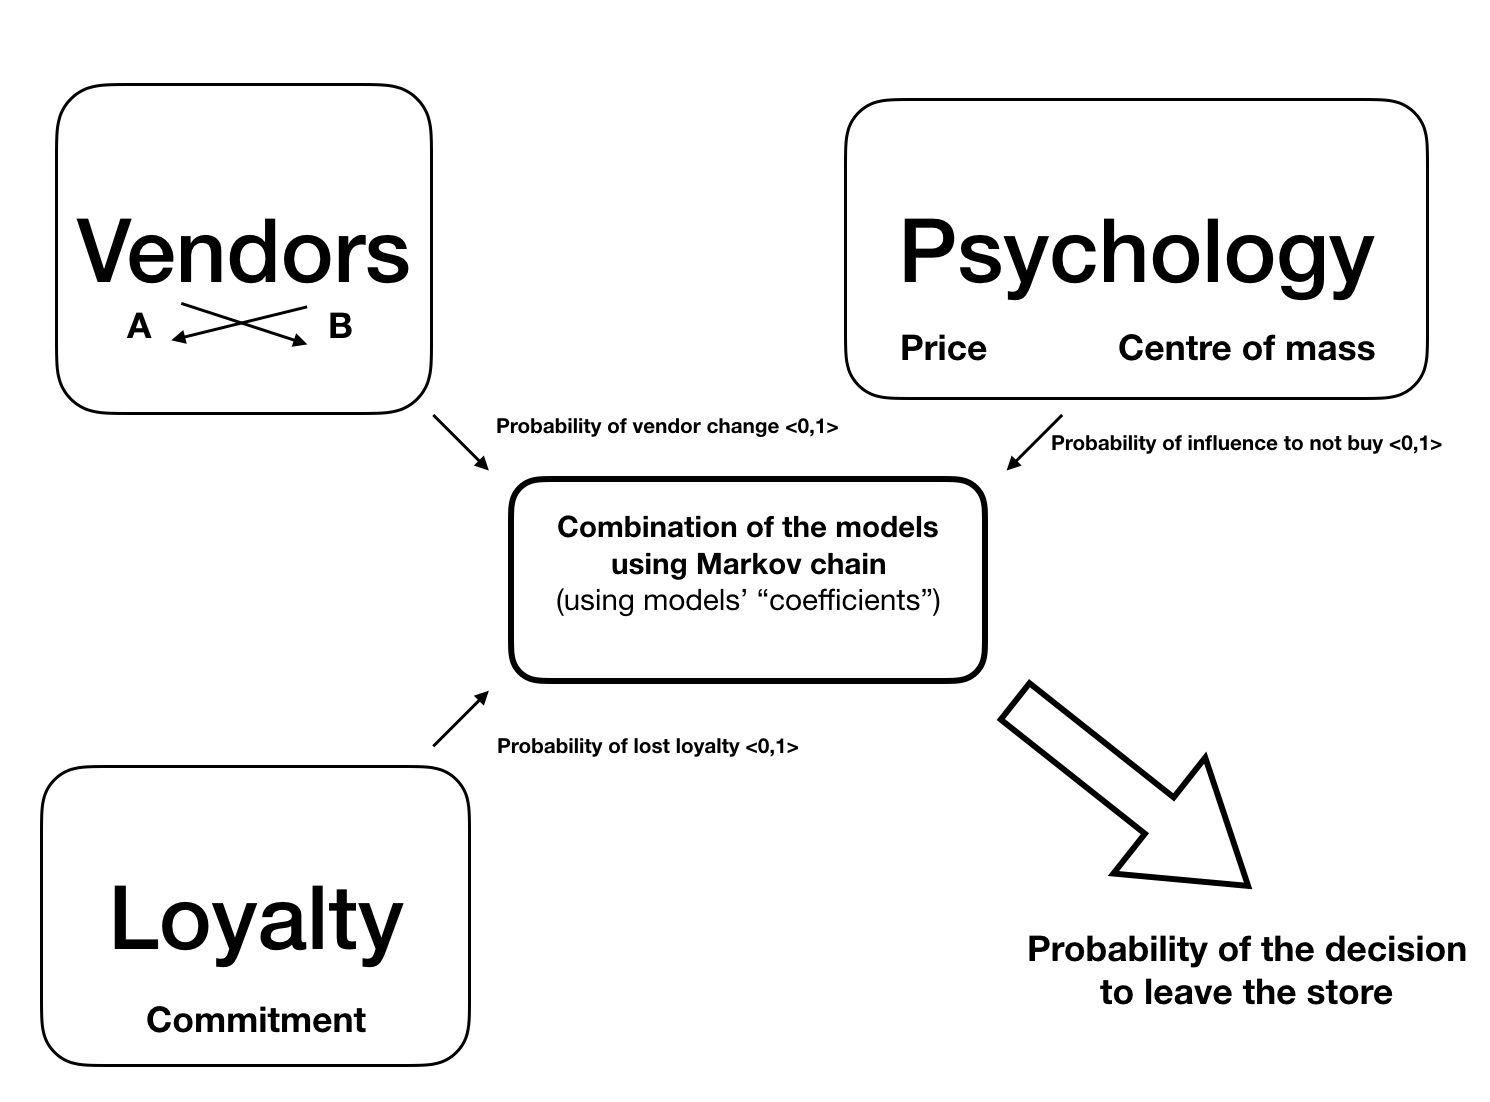
\includegraphics[width=140mm]{computation_schema.png}
    \end{center}
    \caption{Computation flow and interactions between models}
    \label{Model schema with interaction}
\end{figure}
\\
\subsection{Decision process from sub-models (Hidden markov model)} \label{sec:decision}
In a Hidden Markov Model (HMM), we have an invisible Markov chain (which we cannot observe), and each state
generates in random one out of $k$ observations, which are visible to us.
Let’s look at an example. Suppose we have the Markov Chain from above, with three states (snow, rain and sunshine),
$P$ - the transition probability matrix and $q$ — the initial probabilities.
This is the invisible Markov Chain — suppose we are home and cannot see the weather.
We can, however, feel the temperature inside our room, and suppose there are two possible observations: hot and cold.\\
Let us go to our situation.
For our need we will create 3 states model.
States will be:\\
\begin{itemize}
    \item order
    \item not finished order
    \item no order decision
\end{itemize}
With Megaplay s.r.o owner and heureka e-comerce tool calculation data we were set probability wages vector for HMM function like:\\
$$ p_w = \left(\frac{1}{3} & \frac{1}{2} & \frac{1}{9}\right) $$
\\
This vector tells about probabilities for each submodel described in own section~\ref{sec:submodels}
Vector have to be updated to square matrix which is used in HMM function.\\
\begin{equation*}
    P_w =
    \begin{pmatrix}
        \frac{1}{3} & \frac{1}{2} & \frac{1}{9} \\
        \frac{1}{3} & \frac{1}{2} & \frac{1}{9} \\
        \frac{1}{3} & \frac{1}{2} & \frac{1}{9}
    \end{pmatrix}
\end{equation*}\\

\subsection{Preprocessing of input data} \label{subsec:preprocessing}
Data should have to be anonymized \footnote{Data anonymization is a type of information sanitization whose intent is privacy protection.
It is the process of either encrypting or removing personally identifiable information from data sets, so that
the people whom the data describe remain anonymous.} and pseudonymized \footnote{Pseudonymization is a data management
and de-identification procedure by which personally identifiable information fields within a data record are replaced
by one or more artificial identifiers, or pseudonyms.} to keep legal notice of~\cite{gdpr}.
Then we should utilize data to utilized inputs.
This prepared data I will add to the Matlab live script file to be used for prediction.\\
\\
\textbf{Average day visitors for a predicted month}\\
This value was calculated from anonymize user data from Google Analytics tool used their prediction mechanism to get number of future users based on previous a number of visitors.\\
\\
\textbf{Perceived value for psychology model} \label{perceived}\\
This variable is needed for loyalty model~\ref{subsec:model_loyalty} and comes from an open e-commerce compare data provided by Heureka.cz/Heureka.sk internal tool.\\
\\
\textbf{Number of orders 2018 - 2019}\\
Number of orders get from shopycrm.com tool used in Megaplay s.r.o to manage their business processes and store all needed data.\\
\\
\textbf{Unique products sell}\\
This variable is used in Psychology model~\ref{subsec:model_psychology} for Price aspect calculation~\ref{eq:26}.\\
\\
\textbf{Customer satisfaction} \label{customerSat}\\
This value is provided by Heureka open data, and it's a calculated value from the all customer reviews of the store.\\
\\
\textbf{Margin}\\
The retail margin percentage measures the retail margin as a percentage of the retail price.
This measurement gives you a context for the retail margin.
For example, if you have a 5~€ retail margin on two different products, but one costs 150~€ and next one costs 10~€, the second product would have a much higher retail margin percentage.\\
\\
\textbf{Number of product order each day $Q_i$}\\
This is a calculated value from shopycrm.com about number of product order for each one.
It's used in Psychology model~\ref{subsec:model_psychology}. \\
\\
\textbf{Quality index $Q_1$}\\
This is vendor quality index provided by Heureka open data.
This is a power/strength of the store.
Higher number mean that for a customer is more difficult to leave the store and go to another online store.\\
\\
\textbf{Vendor coefficients $\beta, \gamma, \delta$} \label{vendorCoeff}\\
This three coefficients are used as weight for vendor model~\ref{subsec:model_vendors} and was set with cooperation with Megaplay s.r.o owner for their industry.
It's represent the relation between vendor prices and vendor quality.\\
\\
\begin{table}[h!]
    \begin{center}
        \begin{tabular}{ | l | c |}
            \hline
            {\textbf{Variable name}} & \textbf{Result}\\
            \hline
            average day visitors for a predicted month $U_a$& 2357 \\
            perceived value for psychology model & 0.87 \\
            number of orders 2018 - 2019 $O_c$ & 26 530 \\
            Unique products sell $U_p$ & 11048\\
            Customer satisfaction & 90\%\\
            Margin & 0.27\\
            $Q_i$ & 4.12\\
            $Q_1$ & 0.94\\
            Vendor coefficients: & \\
            $\beta$ & 0.7\\
            $\gamma$ & 0.7\\
            $\delta$ & 0.85\\
            \hline
        \end{tabular}
    \end{center}
    \caption{Coefficient data from Megaplay s.r.o}
    \label{megaplay_data}
\end{table}
\\
\begin{table}[h!]
    \begin{center}
        \begin{tabular}{ | l | c |}
            \hline
            {\textbf{Variable name}} & \textbf{Equation}\\
            \hline
            number of visitors 1/2020 & $31 * U_a$\\
            average earn per order & $\sum Income / O_c$\\
            \overline{Q} & $1/U_p * (U_p/ O_c)$\\
            \overline{P} & $1/U_p * margin$\\
            trust & $1/O_c * O_c/U_a$\\
            \hline
        \end{tabular}
    \end{center}
    \caption{Calculated data from Megaplay s.r.o}
    \label{megaplay_data_equation}
\end{table}
\\
\section{Submodels for Customer behavior model} \label{sec:submodels}
\subsection{Vendors} \label{subsec:model_vendors}
For simplification, we will take to account only a two vendors market share, without 100\% domination, because of on a real
market is 100\% monopole unlikely see and then we will be reflected only main competitor.
From that condition it is evident that for market dominate vendor it will return false positive results.
Our model is based on equations from Brands section~\ref{eq:10} and from those equations we will get probability of vendor change from
vendor $A$ to vendor $B$ and if the vendor $B$ will have more strength than vendor $A$ it will break the computation and customer
will leave our store without successfully completing buy process.
Results of this computation wil be probability for each iteration of buy process simulation in an interval $<0,1>$.
Data for this model will comes from open data provided by google.com, heureka.cz/heureka.sk and national governments.
That data will be combined with calculated price indexes downloaded from shopycrm.com tool.
\\
\begin{equation} \label{eq:24}
\alpha_{xy} = \beta H(P_x-P_y) + \gamma H(Qx-Qy) + \delta H(Px-Py)H(Q_x - Q_y)
\end{equation}
\\
where $\beta, \gamma, \delta$ are non-negative~\ref{vendorCoeff}.
\\
\begin{itemize}
    \item $P$ is prices of vendors products
    \item $Q$ is a quality index of vendor
    \item $H$ is a Heaviside function which will be calculated by~\ref{eq:24}.
\end{itemize}
\\
\begin{eqnarray} \label{eq:25}
H(s) = 1, s > 0 \\
H (s) = 0, s \leq 0
\end{eqnarray}
\\
\subsection{Psychology} \label{subsec:model_psychology}
Psychology aspect is trying to simulate customer behavior in thee situation like a prices aspect, society influenced, mood aspect, actual needs
and so on.
In this model we will simplify only for price effect~\ref{subsubsec:model_psychology_price} and center of mass effect~\ref{subsubsec:model_psychology_mass}
\subsubsection{Price aspect} \label{subsubsec:model_psychology_price}
\begin{equation} \label{eq:26}
\overset{-}{Q} = \frac{1}{n_p} \sum_{i=1}^{n_p} Q_i
\end{equation}
\\
\begin{itemize}
    \item $Q_i$ number of orders for product $i$ per day divide amount of orders per same day, prom interval $<0,1>$
    \item $n_p$ number of products in store
\end{itemize}
\\
\begin{equation} \label{eq:27}
\alpha_{ij} = \frac{C+max(Q_j, \overset{-}{Q})}{C+max(Q_i, \overset{-}{Q})}
\end{equation}
\\
Coefficient C is used to be $\alpha_{ij}$ always positive.
\subsubsection{Center of mass aspect} \label{subsubsec:model_psychology_mass}
Center of mass aspect is applied as a part of sociology to our psyhology model.
Marketers use it to manipulate with customers in global way.
Like a black friday, Cyber monday etc., in that days stores manipulate with our psychology by discount prices.
\\
\begin{equation} \label{eq:28}
\overset{-}{P} = \frac{1}{n_p} \sum_{i=1}^{n_p} P_i
\end{equation}
\begin{itemize}
    \item $P_i$ is defined as product price minus retail recommend price divide average price
    \item $n_p$ number of products in store
\end{itemize}
\\
\begin{equation} \label{eq:29}
\alpha_{ij} = \frac{C+max(P_j, \overset{-}{P})}{C+max(P_i, \overset{-}{P})}
\end{equation}
\\
This model returns probability for customer decision to make action from interval $<0,1>$.
\\
\subsection{Loyalty} \label{subsec:model_loyalty}
This models is based on Luarn \& Lin research~\cite{luarn} and we change theirs model for our needs.\\
\begin{equation} \label{eq:30}
L = \frac{R+Z}{Z}
\end{equation}
\\
\begin{enumerate}
    \item L ..... probability of whole loyalty model
    \item R ..... probability of separate loyalty model
    \item Z ..... probability of commitment model
\end{enumerate}
\\
As we see on figure~\ref{Loyalty scheme} Loyalty model is consist of all three sub-models (Trust, Customer Satisfaction, Perceived value)
but commitment model consist of only Trust and Customer Satisfaction.
a,b,c,d,e .... weight coefficient to combine Trust, Customer satisfaction and Perceived value.\\
\newpage
Trust
\begin{equation} \label{eq:31}
T = \frac{1}{n} \sum_{i=1}^{n} O_i
\end{equation}
\\
$O_i$ number of orders divide number of visitors per day $i$
\\
\\
\textbf{Customer satisfaction} (Se defined values in~\ref{customerSat}) are datasets get from open data per each day, individual satisfaction.
For simplified the situation we will use average satisfaction per whole store.
\textbf{Perceived value} (Se defined values in~\ref{perceived}) is subjective value, which depend on a strength of the store.
\subsubsection{Commitment and Loyalty} \label{subsubsec:model_loyalty_commitment}
\textbf{Commitment} is making the actual choice every day or other period basis to keep up with something e.g. a relationship, personal goal, a task, etc.
We would have to hold ourselves accountable to keep a commitment to something or someone.
Similarly, being loyal involves holding ourself accountable as well.
Against of \textbf{Loyalty} which is usually seen as a character trait rather than a conscious decision.
This model return probability for customer decision to not leave the store from interval $<0,1>$.\\
\\
\begin{figure}[h!]
    \begin{center}
        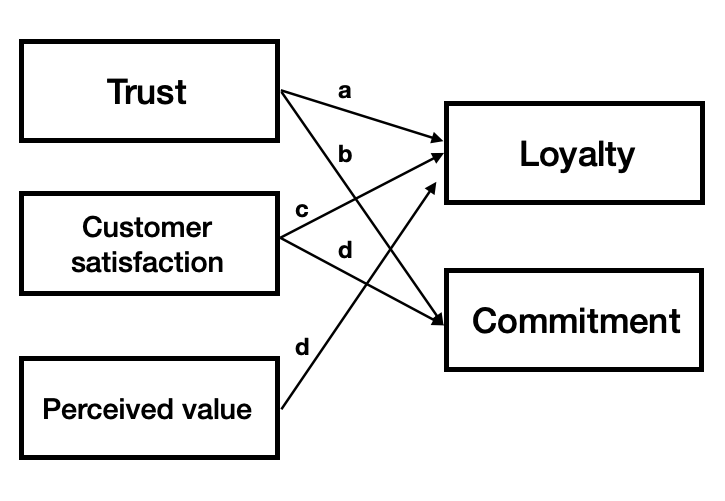
\includegraphics[width=120mm]{loyalty.png}
    \end{center}
    \caption{Computation flow for loyalty and commitment~\cite{luarn}}
    \label{Loyalty scheme}
\end{figure}\\
\newpage
\subsection{Combining models to decision process} \label{subsec:combining_models}
All separates models return probabilities vectors which we update to square matrix which is use as input to Hidden Markov model (HMM) \footnote{Hidden Markov Model (HMM) is a statistical Markov model
in which the system being modeled is assumed to be a Markov process with unobservable (i.e. hidden) states.
The hidden Markov model can be represented as the simplest dynamic Bayesian network.
The mathematics behind the HMM were developed by L. E. Baum and coworkers.
HMM is closely related to earlier work on the optimal nonlinear filtering problem by Ruslan L. Stratonovich,
who was the first to describe the forward-backward procedure.}
These probabilities will be combined with specific weights coefficients to always prevent positives results.
\\
\section{Experiment} \label{experiment}
Let us prepare experiment to test our models. We were prepared three models.
Linear regresion for model:\\
\begin{equation} \label{eq:40}
f(x) = a(\sin(x-\pi))+b((x-10)^2)+c*(1),
\end{equation}\\
with coefficients $a =2.978.10^5,b =1687,c = 1.753.10^6$, polynomial regression for model:\\
\begin{equation} \label{eq:41}
f(x) = p1*x^4 + p2*x^3 + p3*x^2 + p4*x + p5,
\end{equation}\\
with these coefficients: $p1 = 225.1, p2 = -1.059.10^4, p3 =1.596.10^5,\\
p4 = -8.205.10^5, p5 = 2.702.10^6$ and our Customer behavior model, described in figure~\ref{Model schema with interaction}.
These model get us prediction for year 2020.
Prediction period we compared and calculate aberration for each one against real store income from 2020.
Experiment was simulated in Matlab, where internal predefined function was used. See more in section~\ref{subsec:libraries}.
Let see our results in Evaluation section~\ref{evaluation} and Summary section~\ref{summary}.\\
\subsection{Used software, libraries and predefined functions} \label{subsec:libraries}
\textbf{Matlab 2020a}\\
MATLAB (matrix laboratory) is a fourth-generation high-level programming language and interactive environment for numerical
computation, visualization and programming developed by MathWorks.\\
\\
\textbf{Matlab LiveScript}~\cite{livescript}\\
MATLAB live scripts and live functions are interactive documents that combine MATLAB code with formatted text, equations,
and images in a single environment called the Live Editor.
In addition, live scripts store and display output alongside the code that creates it.\\
Use live scripts and functions to:\\
\begin{itemize}
    \item Visually explore and analyze problems
    \item Share richly formatted, executable narratives
    \item Create interactive lectures for teaching
\end{itemize}\\
\\
\textbf{Matlab Curve Fitting Tool}\\
The Curve Fitting Toolbox provides a collection of GUIs and M-files.
With the toolbox we are able to data preprocessing such as sectioning and smoothing, parametric and nonparametric data fitting,
fit statistics to assist you in determining the goodness of fit,analysis capabilities such as extrapolation, differentiation, and integration
A graphical environment that allows you to explore and analyze data sets and fits visually and numerically.\\
\textbf{hhmgenerate}~\cite{hhmgenerate}\\
The function $hmmgenerate$ begins with the model in state 1 at step 0, prior to the first emission.
The model then makes a transition to state $i_1$, with probability $T_{1i_1}$, and generates an emission $a_k_1$ with probability $E_{i_1k_11}$.
$hmmgenerate$ returns $i_1$ as the first entry of states, and $a_k_1$ as the first entry of seq.
$[seq,states] = hmmgenerate(len,TRANS,EMIS)$ takes a known Markov model, specified by transition probability matrix $TRANS$ and emission probability matrix $EMIS$,
and uses it to generate:\\
\begin{itemize}
    \item A random sequence seq of emission symbols
    \item A random sequence states of states
\end{itemize}
The length of both $seq$ and $states$ is $len$.
$TRANS(i,j)$ is the probability of transition from state $i$ to state $j$.
$EMIS(k,l)$ is the probability that symbol $l$ is emitted from state $k$.\\
\\
\textbf{hhmviterbi}~\cite{hhmviterbi}\\
The function $hmmviterbi$ begins with the model in state 1 at step 0, prior to the first emission.
hmmviterbi computes the most likely path based on the fact that the model begins in state 1.
$STATES = hmmviterbi(seq,TRANS,EMIS)$ given a $sequence, seq$, calculates the most likely path through the hidden Markov model
specified by transition probability matrix, $TRANS$, and emission probability matrix $EMIS$. $TRANS(i,j)$ is the probability of transition from state $i$ to state $j$.
$EMIS(i,k)$ is the probability that symbol $k$ is emitted from state $i$.\\
\\
\textbf{shopycrm.com}\\
Online CRM application focused on e-commerce stores which provides all store workflows and get precalculated data which we will use for our models to simplify the prediction calculation.
\newpage
\subsection{Linear and Polynomial regression} \label{sec:baseline}
Let use Matlab Curve fitting tool to solve our linear and polynomial models as you can see on figure~\ref{cftool}, this predefined tool calculate coefficient for and then
the prediction in Matlab Live script was done as we see on figure~\ref{predict}
These two models was trained on income data from years 2018 and 2019.
\begin{figure}[h!]
    \begin{center}
        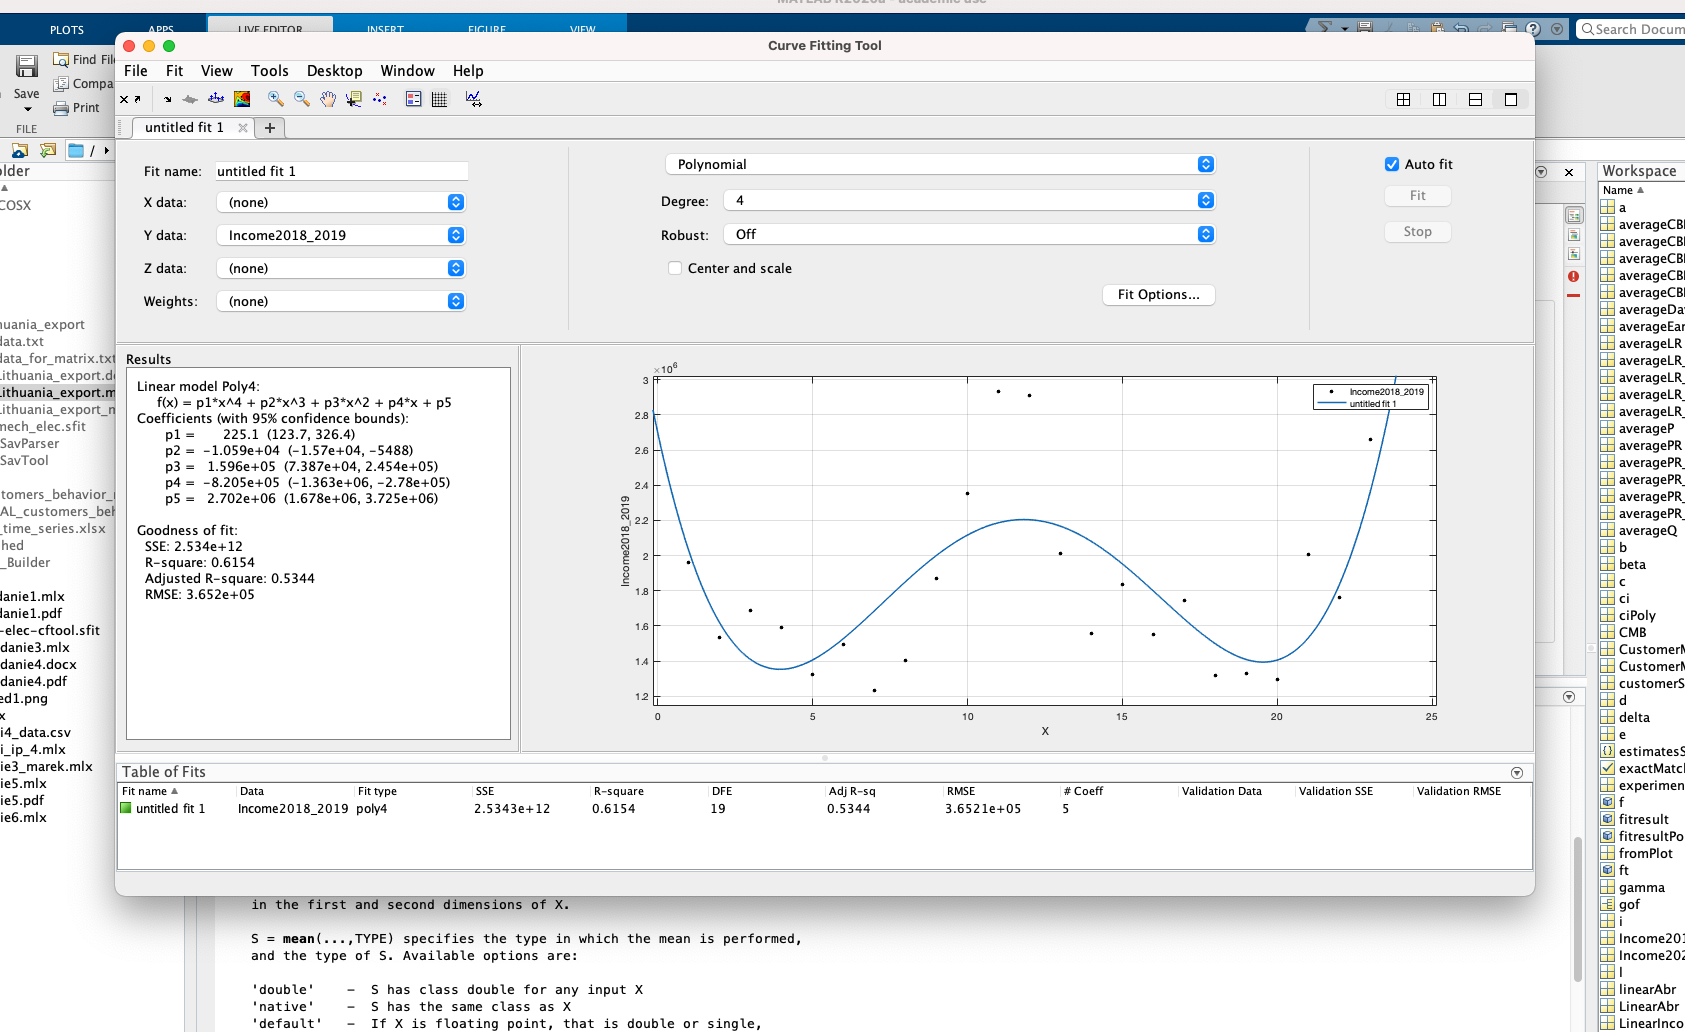
\includegraphics[width=90mm]{cftool.png}
    \end{center}
    \caption{Fitting the data with cftool~\cite{luarn}}
    \label{cftool}
In the next step prediction for year 2020 was made. For prediction we use different mechanism for each model.
The first linear model Matlab's $predint$ function used to get prediction results from previous fitting function.
The second one used other approach.
Trained and prepared polynomila model was compared with real data to see the aberrance. Plotting function was used to see the results.
At a first glance we can se that the results from the models are different. The first linear model with trigonomic function
is not really god in real income results but very interesting result for trend prediction was produced.
In contrast with polynomial model which much better in absolut income results, but worst in trend prediction.
\end{figure}\\
\begin{figure}[h!]
    \begin{center}
        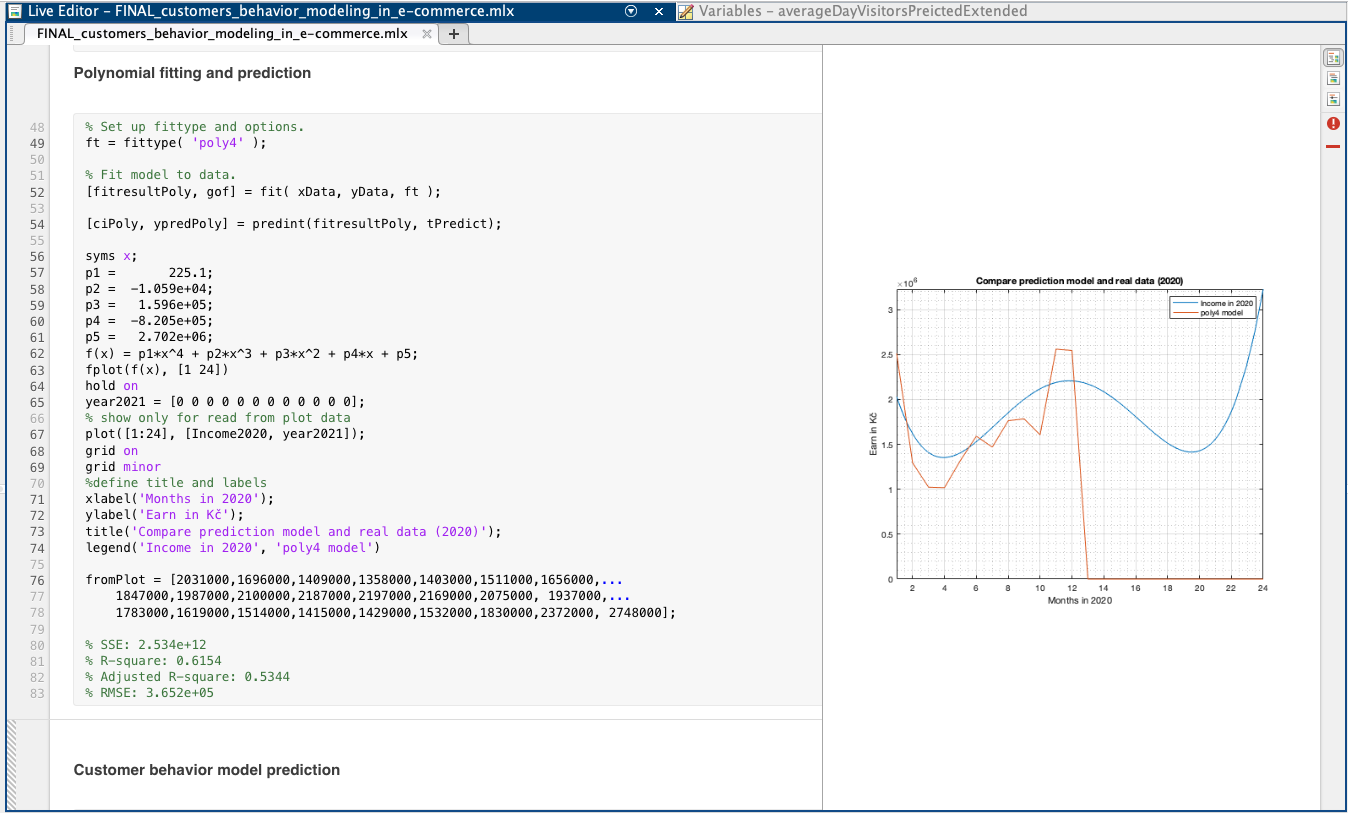
\includegraphics[width=80mm]{predict.png}
    \end{center}
    \caption{Predict income data in live script~\cite{luarn}}
    \label{predict}
\end{figure}\\
\subsection{Customer behavior model} \label{sec:cbm}
Our prediction script is finally written in Matlab Live script with predefined constants based on Megaplay s.r.o data,
but for modeling and dynamic prediction are used Live scripts Controls so in the script we are able to easily set all constant to model for simulate different situations.
Let see the function of our prepared model.
In the first step model get predefined data from inicial part (See more in sectin~\ref{subsec:preprocessing}).
This precalculated data entered calculation loop.
Next loop read the value of predefined number of customers in each period and simulated the virtual customer bavior in order process in the next steps:
\begin{enumerate}
    \item get probability from Vendor submodel
    \item get probability from Psychology submodel
    \item get probability from Loyalty submodel
    \item combine submodels data in Hidden Markov model
    \item read invisible states by Viterbi algoritm
    \item check result matrix produced by viterbi and save the number of success orders
    \item calculate prediction income
\end{enumerate}\\
Whole prediction is made 10 times and the final result is arithmetic mean from this ten times run to random deviation be removed.
We can see model situation in~\ref{apendixc} and that results is described in the final summary~\ref{summary} as results from previous models from section~\ref{sec:baseline}.
\subsection{Using random values} \label{subsec:rand}
In our model random generated variables was used to simulate situations from real store where the user can compare with other store in the different situation.
This other stores and situation should be better or worst to actual store.
To improve results should be better that real competitors' data from each store was used, but is not simple to get them.
This random variables are used as a simplification of that situation.
\subsection{Compare results} \label{subsec:matlab}
Lets us defined the method to compare our models results.
Absolute number of income value prediction is not to represent and important for the store owners, so we were calculated
the aberration for each month prediction and then easily calculate quarterly and yearly results.
\begin{equation} \label{eq:42}
A = ((R - P)/P) * 100,
\end{equation}\\
for predict a situation where real income is higher than prediction or for opposite situation:
\begin{equation} \label{eq:43}
A = ((P - R)/R) * 100,
\end{equation}\\
where $A$ is aberration in percent for real income $R$ and predicted income $P$.
